\documentclass[12pt]{report}
\usepackage{amsmath}
\usepackage{graphicx}
\usepackage{hyperref}
\usepackage[utf8]{inputenc}
\usepackage{listings}

\title{CSU44053 Computer Vision}
\author{Finding bookshelves and recognising books \\ Séamus Woods \\ 15317173}
\date{19/11/2019}

\begin{document}
\maketitle
\newpage

\section{Question}
(a) Given images of bookshelves (such as those shown below), develop a system to locate the shelves on which the books are standing. Your solution must consist of a series of computer vision techniques and the technical details of the techniques used must be provided.
\begin{center}
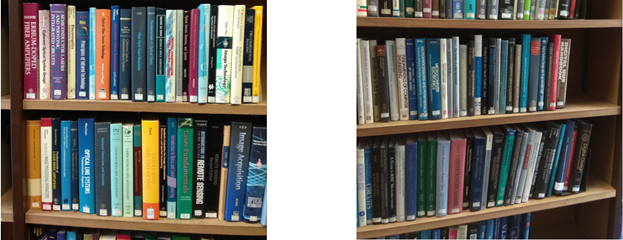
\includegraphics[scale=1]{Bookcases.png}
\end{center}
(b) Describe Template Matching and the Scale Invariant Feature Transform (SIFT) and discuss the issues of applying both of these techniques to the problem of recognising individual books, assuming that you have already located the bookshelves.  Include a discussion of which of these techniques is more appropriate.  You must provide technical details of the both of the techniques.  


\newpage
\section{Answer}
\subsection{Part A}
A brief summary of my method, is to convert the image from RGB colour space to grayscale. Then performing some kind of edge detection, like adaptive thresholding, to get a binary image. Then I think we could use a Hough transform for lines, and the lines with the most amount of intersections would be our shelves.
\newline
The grayscale image is the luminance of a colour image is the luminace at every point of the colour image. From RGB this comes to $Y = 0.299R + 0.587G + 0.114B$, where $Y$ is the luminance. I believe this comes from the Bayer pattern. 
\newline
The reason for getting the grayscale is so that we can get a binary image from it. Though we can use multi-spectral thresholding, it's easier to work with binary images, and there's no practical reason to be concerned with the colour with this problem. I chose to use adaptive thresholding, because from experience I've found it yields the best results. Adaptive thresholding uses multiple thresholds for an image instead of a single global threshold. The algorithm for adaptive threshold is: 
\begin{itemize}
\item Split original image into sub images.
\item Calculate an appropriate threshold for each sub image.
\item Calculate a threshold for every pixel using bilinear interpolation.
\end{itemize}
Sometimes we can have issued with adaptive thresholding where some points may be very dark, but we can fix this by ensuring that threshold values don't vary significantly across the image. 
\newline
Now that we have a binary image, we can use a Hough transform for lines. Hough Transform is a popular technique to detect any shape, if you can represent that shape in a mathematical form. It returns the probability of the existence of some feature, in our case the probability that there is a line. The algorithm is as follows:
\begin{itemize}
\item Initialise all cells $(s, \theta)$ in the Hough space accumulator to 0.
\item For every edge point in the image space $(i,j)$:
	\begin{itemize}
	\item Increment the points as determined using $s = i.cos(\theta) + j.sin(\theta).$ (Alternative for of the line equation)
	\end{itemize}
\item Search for local maximums in the Hough space accumulator. 
\end{itemize}
Now that we have all of the probable lines within the image, my thinking is that the lines with the most amount of intersections will be our shelves. An image should explain this a lot better.
\begin{center}
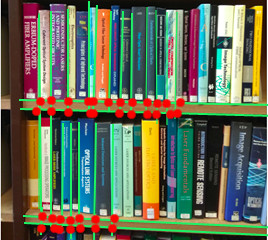
\includegraphics[scale=1]{Bookcases_found.jpg}
\end{center}
So in an ideal world, our hough lines would detect the lines in between all books, and the lines of the shelves. The lines of the shelves would have the most amount of intersections of any other lines in the image, we could do some kind of threshold for amount of intersections in a line. Then we could distinguish which lines belong to which shelves by measuring the distance between lines (e.g. the distance between the top and bottom lines of a shelf would be far less than the distance between the bottom and top of two different shelves).

\subsection{Part B}
\subsubsection{Template Matching}
Template Matching is a very simple technique where a sub-image is search for within an image. It can be quite good under certain circumstances, but does fail often if the image quiality is poor or the object you're looking for is quite similar to other objects in the scene. For example if you were looking for the character 'D', it's very likely that the number '0' would score quite high as a match. The algortihm for template matching is: 
\begin{itemize}
\item For every possible position $(i,j)$ of the object in the image:
\begin{itemize}
\item Evaluate a matching metric and store it in a matching space: $M(i,j)$.
\end{itemize}
\item Search for a local maxima or minima in the matching space above a threshold T.
\end{itemize}
There are a few matching metrics that we can use, among which are square differences and cross correlation. The formula for cross correlation would be:
\begin{center}
$D_{CrossCorrelation} (i,j) = \underset{(m,n)}{\sum} f(i+m, j+n) . t(m,n)$
\end{center}

\subsubsection{SIFT}
SIFT (Scale Invariant Feature Transform) isn't a recognition technique in itself, but a method of extracting features from images, to be used for recognition. Usually for recognition, we would use SIFT to extract features, map those features to other objects, Hough transform to identify clusters of features that come from the same object, and then something like chamfer matching. It is invariant to scaling and rotation and partly invariant to illumination and viewpoint changes. This is a significant step forward from typical corner detectors such as Moravec or Harris. SIFT features are extracted in a number of stages:
\begin{itemize}
\item Scale space extrema detection.
\begin{itemize}
\item Image is condidered at multiple scales simultaneously in order to be invariant to scale.
\item Extrema are located within these scaled images by convolving the image with a number of Gaussians.
\item Potential stable keypoints are found by considering the Difference of Gaussian functions across the various scale spaces.
\end{itemize}
\item Accurate keypoint location.
\begin{itemize}
\item Data is modelled locally using a 3D quadratic and then interpolated max/min can then be found.
\item Low contrast keypoints are discarded. This is evaluated from the curvature of the 3D quadratric.
\end{itemize}
\item Keypoint orientation assignment
\begin{itemize}
\item Used to make features rotation invariant.
\item Scale of the keypoint is used to select Gaussian smoothed image with the closest scale.
\item Creates orientation histogram, weighted by gradient magnitude and distance to they keypoint location.
\item Highest peaks is used to define the keypoint orientation.
\end{itemize}
\item Keypoint descriptors.
\begin{itemize}
\item We use the blurred image at the closest scale, sampling points around the keypoint orientation.
\item Region around the keypoint is divided into four subregions and a weighted historgram of the orientations is determined for each subregion.
\item Orientations are mapped into relevant bins and all adjoining bins to reduce problems relating to quantisation.
\end{itemize}
\end{itemize}

In order to recognise objects, we need to reduce the amount of features which we use. Three features has been found to be a sufficient amount. 

\subsubsection{Conclusion}
I think that template matching would be the more suitable method to recognise individual books. Given that we have already located the bookshelves, we could do a perspective transform to get a front on view of the shelf and books (By using the coordinates of the shelf and the shelf above). An issue we might face here would be finding the coordinates of individual books. We would need this for template matching. Some of the books are fallen and at an angle, this could also turn out the be an issue. We might misidentify some books because they are so similar with template matching, but we would definitely be able to easily recognise books that are quite different to others, like the brigh orange and yellow books. 
\newline
Using SIFT to recognise individual books might be a little complicated for this specific situation. It would probably detect the corners of all books and some features in the letters, but becase all of the books have these same corners and are using the same alphabet, it might be a little difficult to distinbuish between books. Although, it would solve our problem of having books at an angle since it is invariant to orientation.

\end{document}
